%\documentclass[11pt]{article}
\documentclass{ctexart}
\usepackage{amsmath, amssymb}
\usepackage{geometry}
\usepackage{graphicx}

% Set page margins
\geometry{margin=1in}

\title{Ordinary Differential Equations一般微分方程}
\author{Yang transcribed by Handwriting of Prof Langemann}
\date{07.11.2023}

\begin{document}

\maketitle

\section*{Introduction}
Ordinary differential equations (ODEs) are equations involving derivatives of a function. The solution of an ODE is the function itself. This handout will focus on the separation of variables technique and the consideration of initial value problems (IVPs).

\section*{2.1 变量分离法}
变量分离法是解一阶常微分方程(ODE)的一种方法,该方程可以表示为两个函数的乘积,一个仅依赖于独立变量 \( t \),另一个依赖于因变量 \( y \)。

\subsection*{方法}
给定一个形如的ODE:
\[ y' = f(t,y) = g(t)h(y), \]
我们可以分离变量并对两边进行积分:
\[ \int \frac{1}{h(y)} \, dy = \int g(t) \, dt + C. \]

\subsection*{示例}
对于ODE \( y' = 2y/t \),我们对两边进行积分得到:
\[\frac{dy}{dt} = \frac{2y}{t}\]
\[ \int \frac{dy}{dt} = \int \frac{2y}{t} + C , C \in \mathbb{R}\]
这给我们提供了解:
\[ ln|y| = 2ln|t| + C = ln t^2 + C\]
\[|y| = \pm e^c t^2\]
但是 \(y \equiv 0\) 也是一个解

\subsection*{注意事项}
解积分时需要小心,特别是当ODE是自治的(仅依赖于 \( y \))时。

\subsection*{自治ODE}
自治ODE是与时间无关的,可以表示为 \( y' = f(y) \)。它们通常有解,可以可视化为不同轨迹的曲线族,这些轨迹基于初始条件而定。

\subsection*{初值问题 (IVPs)}
根据 **Frobenius'定理**,给定初值条件 \( y(t_0) = y_0 \),讨论ODE的解的存在性和唯一性。

\subsubsection*{**唯一解:** }
如果 \( t \neq 0 \) 且 \( y_0 \neq 0 \),则通过点 \( (t_0, y_0) \) 存在唯一解。

\subsubsection*{**多重解:** }
如果 \( y_0 = 0 \),可能存在多个解,包括平凡解 \( y = 0 \)。

\subsubsection*{**无解:** }
在某些条件下,可能没有满足初值问题的解。

\subsection*{结论}
变量分离法是解一阶ODE的强大技巧。当ODE可以分离为 \( t \) 的函数和 \( y \) 的函数时,考虑初始条件对于确定ODE的解的唯一性和存在性至关重要。
\subsection*{示例}
给定微分方程:
\[ y' = 1 - 2y \]

可以绘制方向场并进行如下的变量分离:

\begin{align*}
\frac{dy}{dt} &= 1 - 2y \\
\int \frac{dy}{1 - 2y} &= \int dt + c \\
\frac{1}{-2} \ln |1 - 2y| &= t + c \\
|1 - 2y| &= e^{-2c} \cdot e^{-2t} \\
1 - 2y &= \pm e^{-2c} \cdot e^{-2t} && \text{(假设 $y = \frac{1}{2}$ 在 $t=0$ 时)} \\
y &= \frac{1}{2}(1 - C e^{-2t}), \quad c \in \mathbb{R}
\end{align*}

给定初始条件 \( y = \frac{1}{2} \) 在 \( t = 0 \) 时,特解为:
\[ y = \frac{1}{2}(1 - C e^{-2t}) \]

考虑替代 \( y' = \frac{dy}{dt} \) , \( \eta = y(\tau) \) 和微分方程:
\[ y(t) - y_0 =\int_{y_0}^{y(t)}d\tau = \int_{t_0}^{t} y'(\tau) \, d\tau \]
这意味着:
\[ \int_{y_0}^{y(t)} \frac{dy}{g(y)} = \int_{t_0}^{t} f(t,y(t)) \, dt \]

使用离散化,我们定义 \( \Delta y_i = y_{i+1} - y_i \) 并近似为:
\[ \int_{y_0}^{y(t)} 1dy \approx \sum_{i=0}^{n-1} \Delta y_i \approx \sum_{i=0}^{n-1} f(t_i,y_i) \Delta t_i \approx 
\int_{t_0}^{t} f (\tau. y(\tau))d\tau\]

我们考虑产品类型的近似:
\[ f(t_i,y_i) \approx g(t_i) \cdot h(y_i) \]
以及
\[ \frac{\Delta y_i}{\Delta t_i} \approx g(t_i) \cdot h(y_i) 或 \frac{\Delta y_i}{h(y_i)} \approx g(t_i) \Delta t_i\]

然后,当 \( n \rightarrow \infty \) 时,我们得到:
\begin{align*}
\int_{y_0}^{y(t)} \frac{dy}{h(\eta)} &= \lim_{n \rightarrow \infty \& \Delta y_i \rightarrow 0} \sum_{i=0}^{n-1} \frac{\Delta y_i}{g(t_i,y_i)} \\
&\approx \lim_{n \rightarrow \infty} \sum_{i=0}^{n-1} g(t_i) \Delta t_i = \int_{t_0}^{t} g(\tau) \, d\tau
\end{align*}


考虑微分方程:
\[ y' = \sqrt{1 - y^2} \]
以及频繁出现的情况:
\[ y' = -a(t)y \]

对于第一个方程,我们展示了分离变量法的步骤:
\begin{align*}
\frac{dy}{dt} &= \sqrt{1 - y^2} \\
\int \frac{dy}{\sqrt{1 - y^2}} &= \int dt + c \\
\arcsin(y) &= t + c \\
y(t) &= \sin(t + c)
\end{align*}

然而,最后一行标记为“错误”表明了解决过程中的误解。

对于频繁出现的情况,解决过程如下:
\begin{align*}
\frac{dy}{dt} &= -a(t)y \\
\int \frac{1}{y} dy &= -\int a(t) dt + c \\
\ln |\frac{y(t)}{y_0}| &=  \int_{t_0}^{t} a(\tau) d\tau + c \\
|\frac{y(t)}{y_0}| &= - e^{\int_{t_0}^{t} a(\tau) d\tau}\\
y(t) &= y_0\cdot e^{-\int a(\tau) d\tau}
\end{align*}

还注意到解决方案永远不会通过 \( y = 0 \),如示意图所示。


示意图包括了 \( y' = \sqrt{1 - y^2} \) 的方向场,指示了 \( y' \geq 0 \) 和 \( y(t) \) 单调增加的区域,以及相轨线分析,显示解受限于 \( -1 < y < 1 \) 的值,永远不会达到值 \( y = \pm 1 \)。


\subsection*{矩阵版本}

对于向量函数 \(\mathbf{q}(t)\),考虑矩阵形式的微分方程:
\[ \mathbf{q}' = -A(t) \mathbf{q} \]
其中 \( A(t) \in \mathbb{R}^{n \times n} \)。

解可以表示为:
\[ \mathbf{q}(t) = e^{-\int_{t_0}^{t} A(\tau) d\tau} \cdot \mathbf{q}_0 \]
其中 \( \mathbf{q}_0 \in \mathbb{R}^n \)。

这涉及到矩阵指数:
\[ e^B = \sum_{k=0}^{\infty} \frac{B^k}{k!} = I + B + \frac{B^2}{2!} + \ldots \]
其中 \( B \in \mathbb{R}^{n \times n} \) ,\( I \) 是单位矩阵。


\section*{2.2 齐次变量的微分方程}

\textbf{定义:} 齐次函数 \( f = f(t,y) \) 的次数 \( n \) 是指:
\[ f(\lambda t, \lambda y) = \lambda^n f(t,y) \]

例如,对于 \( n = 0 \):
\[ f(\lambda t, \lambda y) = f(1, \frac{y}{t}) = g(\frac{y}{t}) \]
其中 \( f \) 仅依赖于 \( \frac{y}{t} \)。

\textbf{要素:}
\[ y' = g\left(\frac{y}{t}\right) \]
即,右侧是次数为 0 的齐次函数。

\textbf{步骤:}
替换 \( u = \frac{y}{t} \) 即 \( y = u \cdot t \)。

然后:
\[ y' = u' \cdot t + u \]
因此:
\[ u' \cdot t + u = g(u) \]
或者等价地:
\[ u' = \frac{1}{t} (g(u) - u) \tag{*} \]

\textbf{结果 (\(*\)):} 使用2.1。

\textbf{示例:}
\[ y' = \frac{t - y}{t + y} = \frac{1}{1 + \frac{y}{t}} = \frac{1}{1 + u} \]
替换 \( u = \frac{y}{t} \) 我们有:
\[ u' \cdot t + u = \frac{1}{1 - u} \]
即,
\[ u' = \frac{1}{t} \left(\frac{1}{1 - u} - u\right) = \frac{1 - u + u^2}{t(1 - u)} \]


\subsection*{分离变量法}

进行分离变量法并应用部分分解(PFD),我们得到:
\[
\int \frac{1-u}{1-u+u^2} \, du = \int \frac{dt}{t} + c
\]


\newpage
\date{15.11.2023}
\subsection*{ODE}

\section*{2.3 一阶线性微分方程Linear Differential Equation of First Order}

一阶线性微分方程的形式如下:
\[
y' + a(t)y = P(t)
\]
其中 \( P(t) \) 是右侧的外部激励。相应的齐次方程是:
\[
y' + a(t)y = 0
\]
非齐次方程是:
\[
y' + a(t)y = P(t) \neq 0
\]

\subsection*{解法步骤}
解非齐次ODE的步骤如下:
\begin{enumerate}
    \item 解齐次ODE \( y_h = C y_t \),其中 \( C \in \mathbb{R} \) 是任意系数。
    \item 通过常数 \( C \) 的变化解非齐次ODE,得到一个特解 \( y_p \)。
\end{enumerate}
通用解为:
\[
y = y_p + C y_t, \quad C \in \mathbb{R}
\]
这是因为线性性质 \( \mathcal{L}\{y_p + C y_t\} = \mathcal{L}\{y_p\} + C \cdot 0 = P \)。

\subsection*{与线性代数的比较}
对于与矩阵 \( A \) 类似的算子 \( \mathcal{L} \),其在 \( \mathbb{R}^{n \times n} \) 中的秩 \( A = n-1 \),核 \( \ker(A) = \{ x \in \mathbb{R}^n \mid Ax = 0 \} \) 的维度为1。也就是说,解空间为 \( x_h = C x_t \)。

对于特解 \( A x_p = b \),通用解为 \( x = x_p + C x_t \)。

\subsection*{示例}
对于 \( A \in \mathbb{R}^{2 \times 2} \),\( A = \begin{pmatrix} 1 & 1 \\ 2 & 2 \end{pmatrix} \),秩 \( A = 1 \),以及 \( A \begin{pmatrix} x \\ y \end{pmatrix} = \begin{pmatrix} b_1 \\ b_2 \end{pmatrix} \),计算 \( A \) 的核 \( \ker(A) \) 和特解 \( x_p \) 如下:

核 \( \ker(A) = \{ x \in \mathbb{R}^2 \mid Ax = 0 \} \) 是倍数 \( x_t = (-c, c) \) 的直线。

特解 \( x_p = \begin{pmatrix} \frac{1}{2} \\ \frac{1}{2} \end{pmatrix} \) ,满足 \( A x_p = b \) 如图所示。

\begin{figure}[h!]
\centering
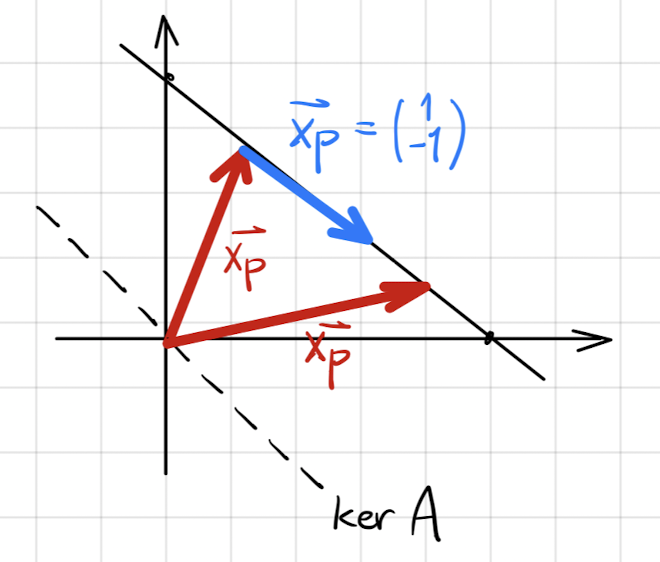
\includegraphics[width=0.5\textwidth]{solution_space.png}
\caption{显示了具有 \( x_p \) 和 \( \ker(A) \) 的解空间的示意图。}
\end{figure}

\subsection*{线性代数中的一些概念}

考虑矩阵 \( A \) 的定义如下:
\[ A = \begin{pmatrix}
    a_{11} & \cdots & a_{1m} \\
    \vdots & \ddots & \vdots \\
    a_{n1} & \cdots & a_{nm}
\end{pmatrix} \in \mathbb{R}^{n \times m} \]

这个矩阵将 \( \mathbb{R}^m \) 映射到 \( \mathbb{R}^n \):
\[ \vec{x} = \begin{pmatrix}
    x_1 \\
    \vdots \\
    x_m
\end{pmatrix} \quad \text{满足} \quad A\vec{x} \]

线性方程组由 \( A\vec{x} = \vec{b} \) 给出。

\subsection*{示例}
对于系统
\[ \begin{pmatrix}
    1 & 1 \\
    3 & 4
\end{pmatrix} \begin{pmatrix}
    x_1 \\
    x_2
\end{pmatrix} = \begin{pmatrix}
    5 \\
    17
\end{pmatrix} \]
我们有唯一的解空间。解为
\[ \begin{pmatrix}
    x_1 \\
    x_2
\end{pmatrix} = \begin{pmatrix}
    3 \\
    2
\end{pmatrix} \]

对于系统
\[ \begin{pmatrix}
    1 & 1 \\
    3 & 3
\end{pmatrix} \begin{pmatrix}
    x_1 \\
    x_2
\end{pmatrix} = \begin{pmatrix}
    5 \\
    14
\end{pmatrix} \]
没有解。

然而,对于
\[ \begin{pmatrix}
    1 & 1 \\
    3 & 3
\end{pmatrix} \begin{pmatrix}
    x_1 \\
    x_2
\end{pmatrix} = \begin{pmatrix}
    5 \\
    15
\end{pmatrix} \]
并且 \( A\vec{x} \neq \vec{0} \),我们有解空间。

\subsection*{解空间}
集合
\[ M = \left\{ \begin{pmatrix}
    x_1 \\
    x_2
\end{pmatrix} = \begin{pmatrix}
    5 \\
    0
\end{pmatrix} + c \begin{pmatrix}
    1 \\
    -1
\end{pmatrix} \right\} \in \mathbb{R}^2 \]
包括 \( \vec{x}_p \)(特解)和 \( \vec{x}_t \)(平凡解)。

\subsection*{A的核}
矩阵 \( A \) 的核定义为:
\[ \ker(A) = \left\{ \vec{x} \mid A\vec{x} = \vec{0} \right\} \]

\subsection*{示例}
微分算子 \( \frac{d}{dt} \) 的核是常数函数,因为常数的导数是0,因此核的维度为1。

\subsection*{A的像}
矩阵 \( A \) 的像定义为:
\[ \text{im}(A) = \left\{ \vec{y} \mid A\vec{x} = \vec{y} \right\} \]


\subsection*{一阶线性常微分方程的解法}

\subsection*{齐次方程}
对于齐次方程
\[ \frac{dy}{dt} = -a(t)y \]
我们找到积分因子 \( \mu(t) \) 如下
\[ \mu(t) = e^{-\int a(t) \, dt} \]
齐次方程的解为
\[ y_h = C \cdot \mu(t) \]
其中 \( C \) 是任意常数。

\subsection*{常数的变化法}
特解 \( y_p \) 可以通过让 \( C(t) \) 成为 \( t \) 的函数来找到:
\[ y_p = C(t) \cdot \mu(t) \]
将其代入ODE以找到 \( C(t) \) 如下:
\begin{align*}
C(t) \mu(t) + C'(t) \mu(t) y_t + a(t) C(t) \mu(t) &= P(t) \\
C'(t) \mu(t) &= P(t) \\
C(t) &= \int \frac{P(t)}{\mu(t)} \, dt
\end{align*}
ODE的通解为:
\[ y = y_h + y_p = \mu(t) \left( C + \int \frac{P(t)}{\mu(t)} \, dt \right) \]

\subsection*{示例}
对于微分方程
\[ y' + 2y = 1 \]
\begin{enumerate}
    \item 齐次部分 \( y' + 2y = 0 \) 的解为 \( y_h = C e^{-2t} \)。
    \item 对于带有外部激励的非齐次部分,我们通过以下方式找到 \( y_p \):
    \[ y_p = C(t) e^{-2t} \]
    通过对 \( y_p \) 进行微分并代入ODE,我们得到 \( C(t) \) 和因此 \( y_p \)。
\end{enumerate}
ODE的通解为:
\[ y = y_p + C y_h = \frac{1}{2} + C e^{-2t}, \quad C \in \mathbb{R} \]

\subsection*{示例:周期外部激励的微分方程}

考虑微分方程
\[ y' + y = \sin(\alpha t) \]
带有周期性外部激励。对于齐次方程 \( y_h = C e^{-t} \),其中 \( C \in \mathbb{R} \),我们有一个瞬态解 \( y_t = e^{-t} \)。

\subsection*{特解}
对于特解 \( y_p \),令 \( y_p = C(t)e^{-t} \),并按如下方式找到 \( C(t) \):
\[ y_p' = C'(t)e^{-t} - C(t)e^{-t} \]
将其代入微分方程得到
\[ C(t) = \int e^{t} \sin(\alpha t) \, dt = \frac{\sin(\alpha t) - \alpha \cos(\alpha t)}{1 + \alpha^2} e^{-t} \]
因此,特解变为
\[ y_p = \frac{\sin(\alpha t) - \alpha \cos(\alpha t)}{1 + \alpha^2} \]
其系统响应与激励频率 \( \alpha \) 同相。

使用三角恒等式,我们可以表示 \( y_p \) 为
\[ A \sin(\alpha t - \varphi) = A \sin \alpha t \cos \varphi + A \cos \alpha t \sin \varphi \]
其中
\[ A \cos \varphi = \frac{1}{1 + \alpha^2}, \quad A \sin \varphi = \frac{\alpha}{1 + \alpha^2} \]
因此
\[ A^2 = \frac{1}{(1 + \alpha^2)^2} + \frac{\alpha^2}{(1 + \alpha^2)^2} = \frac{1}{1 + \alpha^2} \]
给出我们
\[ \tan \varphi = \alpha \]


\begin{figure}[h!]
\centering
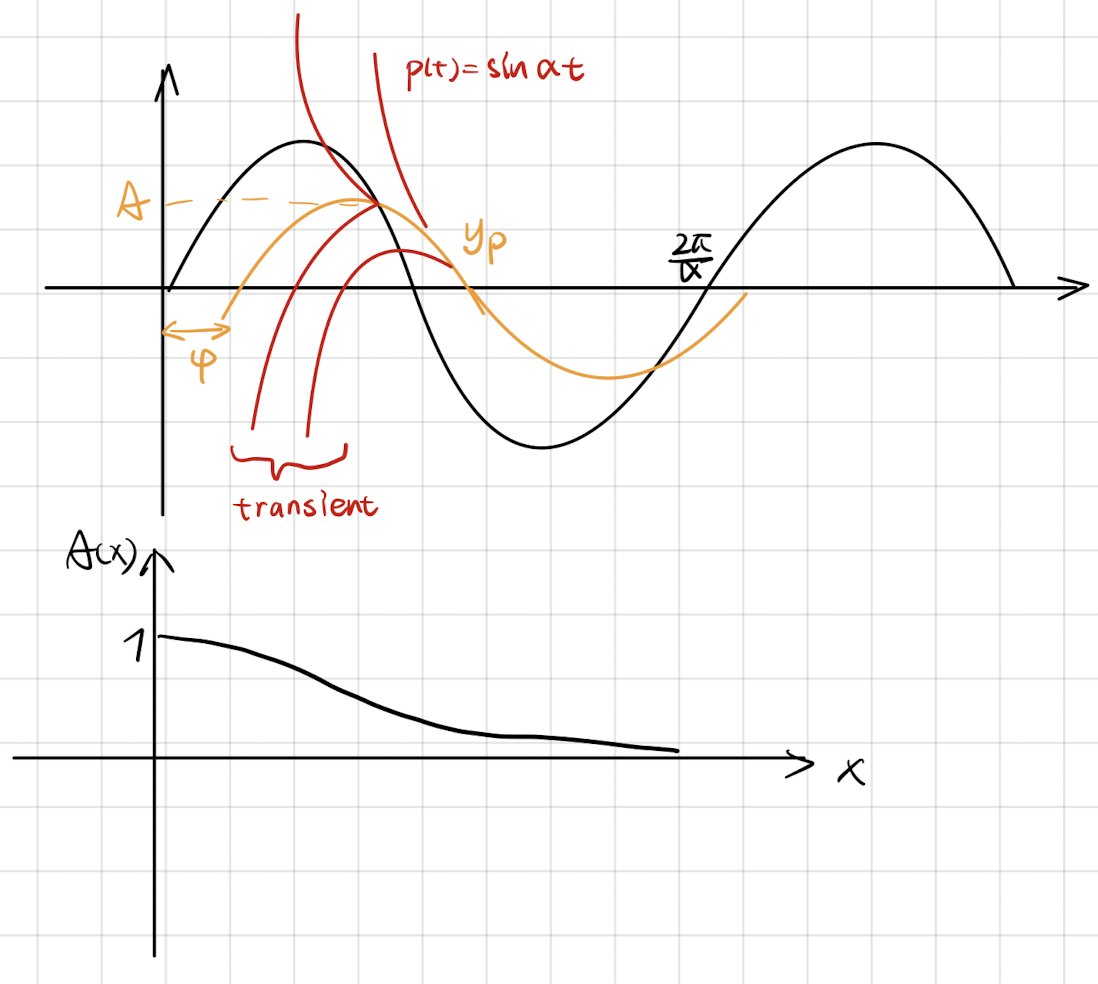
\includegraphics[width=0.5\textwidth]{response_curve.png}
\caption{Response curve showing the transient and steady-state parts of the solution.}
\end{figure}

\section*{2.4 伯努利微分方程}
伯努利微分方程的形式为
\[ y' + a(t)y = p(t)y^n, \quad \text{其中 } n \neq 0,1 \]
可以通过代换 \( u = y^{1-n} \) 来求解,得到
\[ u' + (1-n)a(t)u = (1-n)p(t) \]
这将伯努利微分方程转化为线性微分方程,可以使用第2.3节中描述的方法来解决。

\subsection*{示例:Logistic增长}

考虑Logistic增长微分方程:
\[ y' = y(1-y) \]

这可以重排为:
\[ y' = y - y^2 \]

使用代换 \( u = \frac{1}{y} \),我们得到:
\[ u' = -\frac{y'}{y^2} \]

代入原方程,我们有:
\[ -u' = u - 1 \]
或者等价地
\[ u' = 1 - u \]

解为:
\[ u = 1 + Ce^{-t}, \quad C \in \mathbb{R} \]

回代以找到 \( y \),我们得到:
\[ y = \frac{1}{1 + Ce^{-t}}, \quad C \in \mathbb{R} \]

\begin{figure}[h!]
\centering
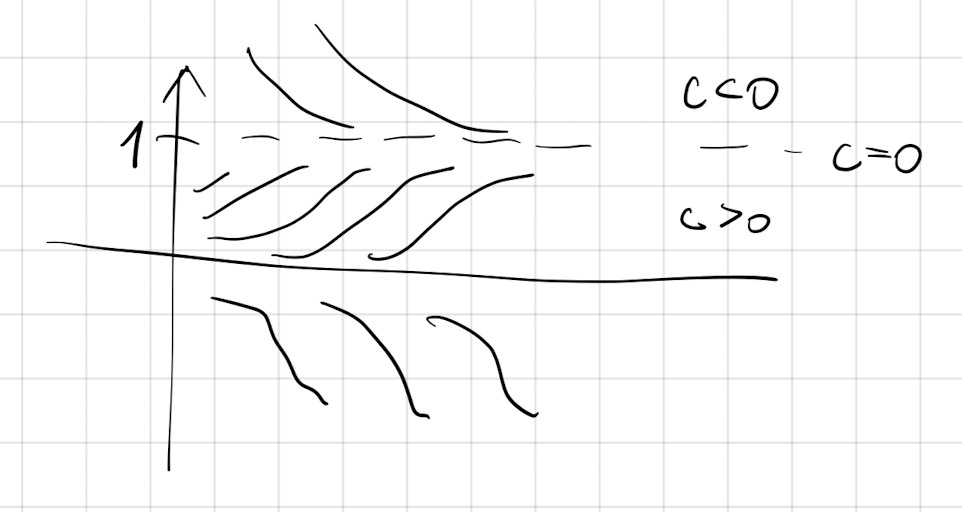
\includegraphics[width=0.5\textwidth]{phase_diagram.png}
\caption{Logistic增长方程的相图。}
\end{figure}


\section*{2.5 精确与完全微分方程}
\subsection*{例子 1}
考虑一个具有弹簧常数 \( k \) 和质量 \( m \) 的无阻尼单质点振子的能量。质点的位置和速度分别用 \( y \) 和 \( v \)(或 \( y' \))表示。

系统的能量 \( E \) 由弹簧的势能和质点的动能之和给出:
\[
E = \frac{1}{2}k y^2 + \frac{1}{2}m v^2 = \Phi(y,v)
\]

由于系统是保守的,能量对时间的总导数为零:
\[
\frac{dE}{dt} = k y \frac{dy}{dt} + m v \frac{dv}{dt} = 0
\]
将方程重写为微分形式,我们有:
\[
k y \, dy + m v \, dv = 0
\]

该系统的相图可以表示为 \( y-v \) 平面中的椭圆,由以下方程描述:
\[
\frac{dv}{dy} = -\frac{k}{m}y
\]

更一般地,对于一个函数 \( \Phi(y,v) \) 在一段时间内保持不变,必须满足以下条件:
\[
0 = \frac{\partial \Phi}{\partial y}(y,v) \, dy + \frac{\partial \Phi}{\partial v}(y,v) \, dv
\]

这引出了一个问题,即是否可以根据给定的函数 \( A(y,v) \) 和 \( B(y,v) \) 来重构 \( \Phi \)。对 \( (A,B)^T \) 的积分条件是必要的:
\[
\frac{\partial A}{\partial v} = \frac{\partial B}{\partial y}
\]

如果要构建关于时间 \( t \) 的 \( \Phi \),则 \( \Phi \) 必须满足以下条件:
\[
0 = \Phi_y(y,v) \, dy + \Phi_v(y,v) \, dv
\]



% 第一个例子
\subsection*{例子 2}
考虑函数 \( A(y,v) = ky \) 和 \( B(y,v) = mv \) 的情况,它们满足可积性条件:
\[
\frac{\partial A}{\partial v} = 0 = \frac{\partial B}{\partial y}
\]
寻找一个函数 \( \Phi \) 使得 \( \frac{\partial \Phi}{\partial y} = A \)。通过积分我们得到:
\[
\Phi = \int A \, dy = \frac{1}{2} k y^2 + C(v)
\]
注意:这里将 \( C(y) \) 改写为 \( C(v) \) 来满足 \( \frac{\partial \Phi}{\partial y} = A \)。

% 检查 B(y,v) = ∂Φ/∂v
接下来,我们验证 \( \frac{\partial \Phi}{\partial v} = B \):
\[
\frac{\partial \Phi}{\partial v} = 0 + \frac{d C(v)}{dv} = mv
\]
从而得出 \( C(v) = \frac{1}{2} m v^2 + C \),其中 \( C \) 是一个常数。

因此,我们找到了 \( \Phi \):
\[
\Phi = \frac{1}{2} k y^2 + \frac{1}{2} m v^2 + C
\]
现在,函数 \( \Phi(y(t),v(t)) \) 的水平集是 \( ky \, dy + mv \, dv = 0 \) 的解集,因为 \( C \) 是任意的。

% 第二个例子
\subsection*{例子 3}
现在考虑一个形式为 \( y(-\frac{1}{x^2}) \, dx + (x + \frac{1}{x}) \, dy = 0 \) 的微分方程,这里 \( A = -\frac{1}{x^2} \) 和 \( B = x + \frac{1}{x} \)。

我们可以通过积分 \( A \, dx \) 来寻找潜在的函数 \( \Phi \):
\[
\Phi = \int A \, dx = y(x - \frac{1}{x}) + C(y)
\]
对 \( \Phi \) 求关于 \( y \) 的偏导得到:
\[
\Phi_y = x - \frac{1}{x} + C'(y) = B
\]
这意味着 \( C'(y) = 0 \),例如我们可以取 \( C = 0 \)。

因此,\( \Phi \) 可以表示为:
\[
\Phi = y(x - \frac{1}{x}) = h
\]
这里 \( h \) 是一个实数常量,表示能量守恒。

% 第三个例子
\subsection*{例子 4}
另一个微分方程 \( y(x^2 - 1) \, dx + (x^3 + x) \, dy = 0 \) 可以写作 \( A = x^2 - 1 \) 和 \( B = x^3 + x \)。但是,这里
\[
\frac{\partial A}{\partial y} \neq \frac{\partial B}{\partial x}
\]
因为 \( \frac{\partial A}{\partial y} = 0 \) 而 \( \frac{\partial B}{\partial x} = 3x^2 + 1 \),所以它不再是精确的微分方程。




\subsection*{微分方程的积分因子与解的存在性和唯一性}

\subsection*{积分因子}
考虑含有积分因子 \( M \) 的方程,使得 \( M\hat{A}dx + M\hat{B}dy = 0 \) 成为精确微分方程。这里 \( \hat{A} \) 和 \( \hat{B} \) 分别对应于原方程中的 \( A \) 和 \( B \),并且有 \( \hat{A}_y = \hat{B}_x \)。

一般偏微分方程(PDE)的形式为 \( M\hat{A}_y = M\hat{B}_x \)。尝试一个解的形式(ansatz),例如 \( M \) 只是 \( x \) 的函数 \( M(x) \)。对于 \( M \),我们有一个常微分方程(ODE):
\[
M(x^{-1}) = M(x(x^2 + x)) + M(3x^2 + 1)
\]

在尝试和失败的过程中,我们发现 \( M \) 不能只是 \( y \) 或 \( x \) 的单独函数,因为这会导致矛盾。

\subsection*{存在性和唯一性}
关于解的存在性和唯一性,我们有皮亚诺(Peano)的存在定理:

简而言之,如果函数 \( f(t,y) \) 是连续的,则解 \( y(t) \) 在整个定义域中存在。

更具体地,如果函数 \( f(t,y) \) 对于 \( t \in [t_0, t_0 + \alpha] \) 和 \( y \in [y_0 - \beta, y_0 + \beta] \) 是连续的,那么初始值问题 \( y' = f(t,y) \),\( y(t_0) = y_0 \) 在 \( t \in [t_0, t_0 + \delta] \) 有解,其中 \( \delta \) 和 \( M \) 由下面的表达式给出:
\[
M = \max_{\substack{t \in [t_0,t_0+\alpha] \\ y \in [y_0-\beta,y_0+\beta]}} |f(t,y)|
\]



\section*{微分方程解的存在性与唯一性}

该图解释了初始值问题的解在有限时间区间长度 \( \beta \) 上的存在性,并且解曲线的斜率由函数 \( M \) 给出。

% 假设你已经将图像保存在名为"image.png"的文件中
\begin{figure}[h]
\centering
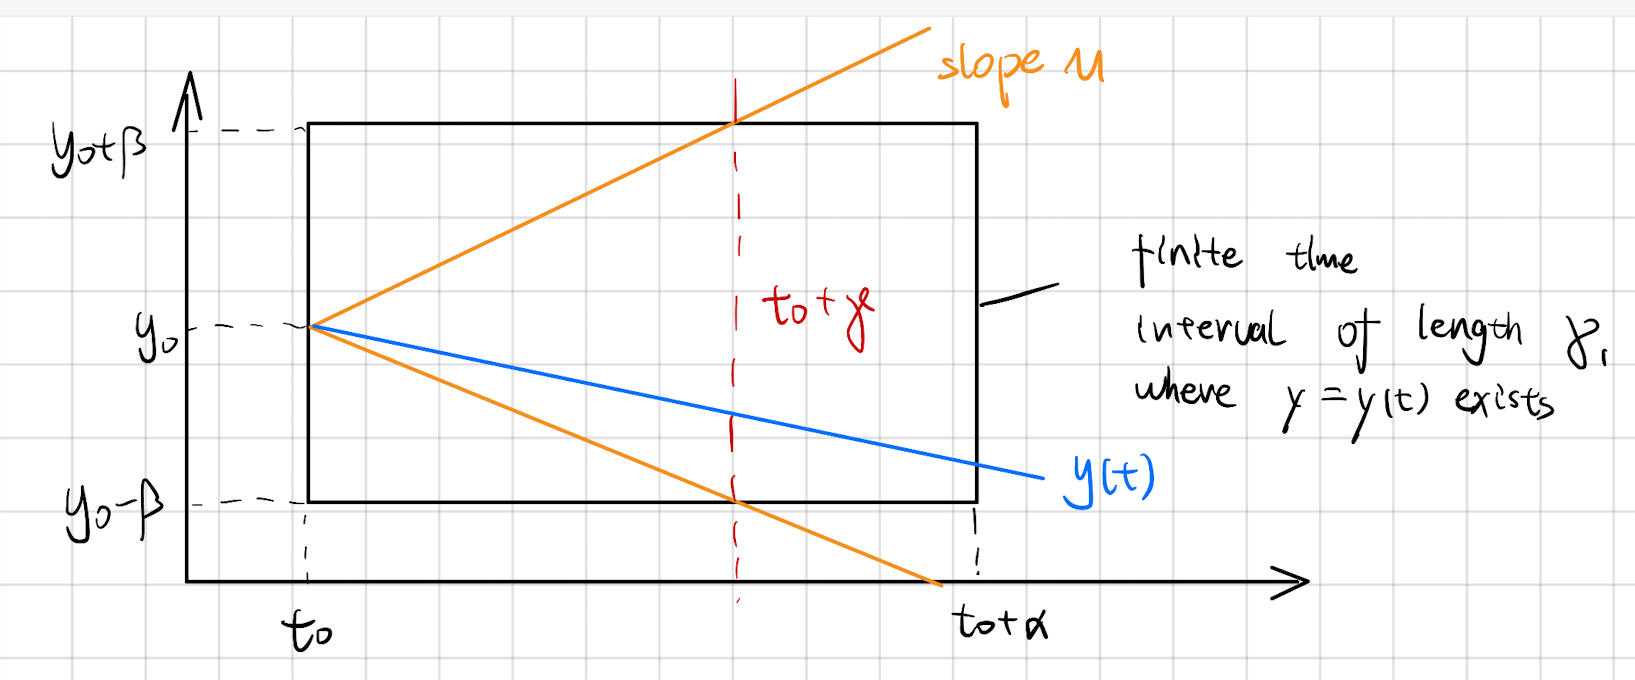
\includegraphics[width=0.8\textwidth]{image.png}
\caption{具有斜率 \( M \) 的解曲线示意图}
\end{figure}

\subsection*{不存在性例子}
如果函数 \( f \) 不连续,我们可能会失去解 \( y \) 的存在性。例如:

\[
y' = 
\begin{cases} 
1 & \text{对于 } y > 0 \\
-1 & \text{对于 } y \leq 0
\end{cases}
\]

这个分段函数在 \( y=0 \) 处没有解,因为解可以朝多个可能的方向发展,如图所示。

\subsection*{非唯一性例子}
函数 \( f \) 的连续性并不能保证解的唯一性。考虑微分方程:

\[
y' = 2 \sqrt{|y|}
\]

在这里,系统必须决定在函数改变方向的点之后如何继续。可以采取多条路径,导致解不唯一。

\[
y(t) = 
\begin{cases} 
-(t-t_0)^2 & \text{对于 } t < t_0 \\
(t-t_0)^2 & \text{对于 } t \geq t_0
\end{cases}
\]

这反映了连续性强定律的违反,即瞬时效应的大小受到原因大小的限制。




\section*{IV 线性常微分方程}

\subsection*{I. 阶数为 \( n \) 的线性常微分方程}
线性常微分方程是由线性微分算子 \( \mathcal{L} \) 定义的,它将 \( [0,T] \) 区间上 \( n \) 次连续可导的函数映射到同一区间上的连续函数:
\[
\mathcal{L}\{y\} = y^{(n)}(t) + a_{n-1}(t)y^{(n-1)}(t) + \cdots + a_1(t)y'(t) + a_0(t)y(t)
\]

\subsection*{II. 线性算子的性质}
算子 \( \mathcal{L} \) 是线性的,因为它满足以下性质:
\[
\mathcal{L}\{\lambda y + \mu z\} = \lambda \mathcal{L}\{y\} + \mu \mathcal{L}\{z\}
\]
其中 \( y,z \in C^n([0,T]) \),\( \lambda, \mu \) 是任意常数。

\subsection*{III. 非齐次与齐次方程}
对于非齐次方程 \( \mathcal{L}\{y\} = p(t) \),齐次方程对应于 \( \mathcal{L}\{y\} = 0 \)。根据叠加原理,\( \mathcal{L}\{y\} = p(t) \) 的通解可以表示为特解 \( y_p \) 和齐次解 \( y_h \) 的和:
\[
y = y_p + y_h
\]
其中 \( y_p \) 是固定的特解,满足 \( \mathcal{L}\{y_p\} = p(t) \),而 \( y_h \) 是任意的齐次解,满足 \( \mathcal{L}\{y_h\} = 0 \)。

\subsection*{IV. 证明}
若 \( y_p \) 和 \( y_h \) 分别是特解和齐次解,那么它们的和 \( y = y_p + y_h \) 也是 \( \mathcal{L}\{y\} = p(t) \) 的解,即:
\[
\mathcal{L}\{y_p + y_h\} = \mathcal{L}\{y_p\} + \mathcal{L}\{y_h\} = p + 0
\]
因此,我们得到 \( y_h = y - y_p \)。

\subsection*{V. 解的任务}
寻找方程的解主要有两个任务:
\begin{enumerate}
  \item 寻找所有的齐次解 \( y_h \),它们满足 \( \mathcal{L}\{y_h\} = 0 \)。
  \item 寻找一个特定的特解 \( y_p \),它满足 \( \mathcal{L}\{y_p\} = p \)。
\end{enumerate}
线性独立的函数 \( y_1, y_2, \ldots, y_n \) 将构成通解的基础。


% 续前面的文档
% ...

\subsection*{线性无关性}
如果函数 \( y_1, y_2, \ldots, y_n \) 线性无关,那么对于任何不全为零的常数 \( \lambda_1, \lambda_2, \ldots, \lambda_n \),方程
\[
\lambda_1 y_1 + \lambda_2 y_2 + \cdots + \lambda_n y_n = 0
\]
只有平凡解,即所有的 \( \lambda_i \) 都必须为零。

如果 \( y_1, y_2, \ldots, y_n \) 线性相关,那么存在不全为零的 \( \lambda_i \) 使得上述方程成立。

\subsection*{定理}
\( \mathcal{L}\{y\} = 0 \) 的通解具有形式
\[
y(t) = c_1 y_1(t) + \cdots + c_n y_n(t)
\]
其中 \( y_1, \ldots, y_n \) 是线性无关的函数,\( c_1, \ldots, c_n \) 是常数。

\subsection*{初值问题(IVPs)的证明}
考虑 \( n \) 个初值问题,其中 \( \mathcal{L}\{y\} = 0 \),并且除了一个初始条件 \( y^{(i)}(0) = 1 \) 之外,其他 \( y^{(j)}(0) = 0 \) (\( i \neq j \))。

例如,对于 \( n = 3 \):
\[
\begin{aligned}
&\mathcal{L}\{y_1\} = 0, \quad \mathcal{L}\{y_2\} = 0, \quad \mathcal{L}\{y_3\} = 0 \\
&y_1(0) = 1, \quad y_2(0) = 0, \quad y_3(0) = 0 \\
&y'_1(0) = 0, \quad y'_2(0) = 1, \quad y'_3(0) = 0 \\
&y''_1(0) = 0, \quad y''_2(0) = 0, \quad y''_3(0) = 1 \\
\end{aligned}
\]
则解可以写为
\[
y = \sum_{i=1}^{n} c_i y_i(t)
\]
满足 \( \mathcal{L}\{y\} = 0 \) 且 \( y^{(i)}(0) = c_i \)。

因为 \( y_1, \ldots, y_n \) 是线性无关的,所以 \( \sum_{i=1}^{n} c_i y_i = 0 \) 只能当所有的 \( c_i \) 都为零时成立。





% 续前面的文档
% ...

\subsection*{Wronskian行列式}
函数 \( y_1, y_2, \ldots, y_n \) 形成向量空间 \( \{ y | \mathcal{L}\{y\} = 0 \} \) 的基,我们称 \( y_1, \ldots, y_n \) 为微分方程 \( \mathcal{L} \) 的基础解系。

Wronskian行列式 \( W(t) \) 定义为:
\[
W(t) = \begin{vmatrix}
y_1(t) & y_2(t) & \cdots & y_n(t) \\
y'_1(t) & y'_2(t) & \cdots & y'_n(t) \\
\vdots & \vdots & \ddots & \vdots \\
y^{(n-1)}_1(t) & y^{(n-1)}_2(t) & \cdots & y^{(n-1)}_n(t)
\end{vmatrix}
\]

如果连续系数的微分方程 \( \mathcal{L}\{y\} = 0 \) 的解 \( y_1, \ldots, y_n \) 满足 \( W(t) \neq 0 \),则它们线性无关。

\subsection*{解的线性无关性判定}
解 \( y_1, \ldots, y_n \) 的线性无关性可以通过Wronskian行列式在某一点 \( t \) 的值来判定。如果 \( W(t) \neq 0 \),则解线性无关;如果 \( W(t) = 0 \),则解可能线性相关。

\subsection*{证明思路}
证明解的线性无关性可以通过考虑线性组合 \( \lambda_1 y_1 + \cdots + \lambda_n y_n = 0 \) 并对其求导来展开。

\subsection*{例子}
考虑 \( y_1 = \sin^2 t \),\( y_2 = \cos^2 t \),\( y_3 = 1 \),并且 \( y_1 + y_2 - y_3 = 0 \) 表明它们是线性相关的。

另一个例子,\( y_1 = t \),\( y_2 = t^2 \),\( y_3 = t^3 \) 是线性无关的,因为它们的Wronskian行列式 \( W(t) \) 在 \( t \neq 0 \) 时不为零。


% ...(前文内容)

\subsection*{寻找特解}
为了寻找微分方程 \( \mathcal{L}\{y\} = p \) 的特解 \( y_p \),我们使用常数变易法。对于已知的线性无关解 \( y_1, y_2, \ldots, y_n \) 满足齐次方程 \( \mathcal{L}\{y\} = 0 \),我们假设
\[
y_p = c_1(t)y_1 + c_2(t)y_2 + \cdots + c_n(t)y_n
\]
其中 \( c_1(t), c_2(t), \ldots, c_n(t) \) 是待定的函数。

我们对 \( y_p \) 进行微分,并将其代入原方程,得到一个关于 \( c_1', c_2', \ldots, c_n' \) 的线性方程组,从而求得 \( c_1(t), c_2(t), \ldots, c_n(t) \)。

\subsection*{例子}
考虑方程
\[
y'' - \frac{6}{t^2}y = t \ln t
\]
其对应的齐次方程为
\[
y'' - \frac{6}{t^2}y = 0
\]
使用欧拉方程的解法,假设 \( y = t^\alpha \) 代入方程,得到特征方程
\[
\alpha(\alpha-1)t^{\alpha-2} - 6t^{\alpha-2}t = 0
\]
解得 \( \alpha_1 = 3 \), \( \alpha_2 = -2 \)。

因此,齐次方程的解为
\[
y_h = c_1t^3 + \frac{c_2}{t^2}, \quad c_1, c_2 \in \mathbb{R}
\]
它们解决了齐次ODE。

现在使用常数变易法,我们假设特解的形式为
\[
y_p(t) = c_1(t)t^3 + c_2(t)\frac{1}{t^2}
\]
进一步求解 \( c_1(t) \) 和 \( c_2(t) \)。

% ...(此处应详细展开计算过程)

最终得到特解 \( y_p \)。



\end{document}
